% =====================================================================
% Spectrogram-Based CNN with Attention for Deepfake Audio Detection
% Brian Stever  |  APCV 485 -- Deep Learning in Cyber  |  Spring 2026
% =====================================================================
\documentclass[11pt, letterpaper]{article}

% --- geometry / spacing --------------------------------------------------
\usepackage[letterpaper, margin=1in, headheight=15pt, headsep=14pt]{geometry}
\usepackage{setspace}
\setstretch{1.05}

% --- typography ----------------------------------------------------------
\usepackage{iftex}
\ifPDFTeX
  \usepackage[T1]{fontenc}
  \usepackage[utf8]{inputenc}
\fi
\usepackage{lmodern}
\usepackage{textcomp}
\usepackage{microtype}
\frenchspacing                                 % single space after period

% --- math / symbols ------------------------------------------------------
\usepackage{amsmath,amssymb}

% --- color palette -------------------------------------------------------
\usepackage{xcolor}
\definecolor{accentink}{HTML}{1B3F6E}   % deep navy used for links + rules
\definecolor{ruleink}{HTML}{2A2A2A}
\definecolor{captionink}{HTML}{222222}

% --- graphics, tables, captions -----------------------------------------
\usepackage{graphicx}
\graphicspath{{figures/}}
\usepackage{booktabs}
\usepackage{array}
\usepackage{tabularx}
\usepackage{makecell}
\renewcommand\theadalign{cb}
\usepackage{float}
\usepackage{placeins}                  % \FloatBarrier
\usepackage{caption}
\captionsetup{
  font=small,
  labelfont={bf,color=accentink},
  labelsep=period,
  textfont=it,
  justification=raggedright,
  singlelinecheck=false,
  belowskip=4pt
}

% --- lists ---------------------------------------------------------------
\usepackage{enumitem}
\setlist[itemize]{leftmargin=1.4em, itemsep=0.25em, topsep=0.25em}
\setlist[enumerate]{leftmargin=1.7em, itemsep=0.25em, topsep=0.25em}

% --- section headings (a touch more elegant than default) ---------------
\usepackage{titlesec}
\titleformat{\section}
  {\normalfont\large\bfseries\color{accentink}}
  {\thesection.}{0.6em}{}
\titleformat{\subsection}
  {\normalfont\normalsize\bfseries}
  {\thesubsection}{0.5em}{}
\titleformat{\subsubsection}
  {\normalfont\normalsize\itshape}
  {\thesubsubsection}{0.5em}{}
\titlespacing*{\section}{0pt}{1.4em}{0.5em}
\titlespacing*{\subsection}{0pt}{1.0em}{0.35em}
\titlespacing*{\subsubsection}{0pt}{0.7em}{0.25em}

% --- header / footer -----------------------------------------------------
\usepackage{fancyhdr}
\pagestyle{fancy}
\fancyhf{}
\renewcommand{\headrulewidth}{0.4pt}
\renewcommand{\footrulewidth}{0pt}
\renewcommand{\headrule}{\color{accentink}\hrule width\headwidth height0.4pt}
\fancyhead[L]{\small\itshape Stever  $\cdot$  Deepfake Audio Detection in Podcast Production}
\fancyhead[R]{\small APCV 485, Spring 2026}
\fancyfoot[C]{\small\thepage\ of \pageref*{LastPage}}
\usepackage{lastpage}

% Title page uses plain style by default -- give it the same minimal feel
\fancypagestyle{titlestyle}{
  \fancyhf{}\renewcommand{\headrulewidth}{0pt}
  \renewcommand{\headrule}{}
  \fancyfoot[C]{\small Final Project Report  $\cdot$  May 2026  $\cdot$  \thepage\ of \pageref*{LastPage}}
}

% --- hyperlinks (subtle academic look) ----------------------------------
\usepackage[
  colorlinks=true,
  linkcolor=accentink,
  citecolor=accentink,
  urlcolor=accentink,
  pdfborder={0 0 0}
]{hyperref}
\usepackage[capitalize]{cleveref}

% --- abstract environment styled like a paper --------------------------
\renewenvironment{abstract}{%
  \begin{center}\bfseries\color{accentink} ABSTRACT \end{center}
  \vspace{-0.4em}
  \begin{quote}\small\itshape\noindent\ignorespaces
}{%
  \end{quote}\vspace{0.5em}
}
\newenvironment{keywords}{%
  \vspace{-0.6em}
  \begin{quote}\small\noindent
  \textbf{\color{accentink}Index Terms.} \ignorespaces
}{%
  \end{quote}\vspace{0.4em}
}

% --- a slightly tighter list inside the abstract -----------------------
\setlength{\parskip}{0.35em}
\setlength{\parindent}{1.2em}

% --- helpful column types for tables -----------------------------------
\newcolumntype{L}[1]{>{\raggedright\arraybackslash}p{#1}}
\newcolumntype{R}[1]{>{\raggedleft\arraybackslash}p{#1}}
\newcolumntype{C}[1]{>{\centering\arraybackslash}p{#1}}

% =====================================================================
\begin{document}
% =====================================================================

% --- title block ---------------------------------------------------------
\thispagestyle{titlestyle}

\begin{center}
{\Large\bfseries Spectrogram-Based CNN with Attention for}\\[0.15em]
{\Large\bfseries Deepfake Audio Detection in Podcast Production}\\[0.4em]
{\color{accentink}\rule{\textwidth}{0.6pt}}\\[1.2em]

{\large Brian Stever \quad \small (Student \#24042080)}\\[0.4em]
{\itshape College of Information Science, University of Arizona}\\[0.15em]
{\itshape Tucson, AZ, USA \quad \texttt{\href{mailto:brianstever@arizona.edu}{brianstever@arizona.edu}}}\\[0.6em]
{\small APCV 485 -- Deep Learning in Cyber\quad$\cdot$\quad Instructor: Dr.\ Shengjie Xu}\\[0.15em]
{\small \today}\\[1.0em]
\end{center}

% --- abstract -----------------------------------------------------------
\begin{abstract}
Deepfake audio creates a practical cybersecurity problem for podcast production, because a familiar voice can act as a brand asset, an identity signal, and an informal trust factor. In this project, I built an end-to-end deep learning detector that classifies audio as bonafide or spoofed from 128-bin log-Mel spectrograms using a convolutional neural network with a Squeeze-and-Excitation channel-attention block. The system uses 16\,kHz mono audio, 4-second clips, podcast-style augmentation, binary classification, and Equal Error Rate (EER) as the headline metric. I trained on the full ASVspoof 2019 Logical Access training partition, selected checkpoints on the full 2019 development partition, and evaluated on the full ASVspoof 2021 Logical Access evaluation set ($n=181{,}566$ trials). On clean 2021 LA, my CNN\,+\,SE detector reached 18.28\% EER, 0.8979 AUC-ROC, 0.9072 accuracy, 0.9479 F1, and 1.66\,ms local Apple-Silicon latency per 4\,s clip. Under podcast-style evaluation stress, EER moved only slightly to 18.48\%, while AUC dropped to 0.8852. A ResNet-18 baseline reached lower EER at 17.21\%; a traditional LFCC-GMM baseline was much weaker at 30.89\%. The main finding is that the full pipeline runs end-to-end and beats a hand-crafted feature baseline by a wide margin, but generalization on the full 2021 LA protocol is genuinely hard and threshold calibration is essential under distribution shift.
\end{abstract}

\begin{keywords}
audio deepfake detection; anti-spoofing; ASVspoof; convolutional neural network; squeeze-and-excitation; podcast production cybersecurity.
\end{keywords}

% =====================================================================
\section{Introduction}\label{sec:intro}

Generative voice systems have made synthetic speech easier to create and harder to dismiss as a novelty. Modern text-to-speech and voice-conversion tools can learn a voice from short clean samples, and podcast hosts publish hours of exactly that kind of audio. For podcast creators, the risk is not just that a fake clip can sound convincing. The deeper issue is that a familiar voice carries trust: a fake episode, ad read, apology, or production instruction can damage the credibility of the person whose voice was cloned, and can trigger downstream contractual or platform-policy consequences.

I took a podcast-production view of deepfake-audio detection because this is the part of the problem closest to my own work. The central premise is that synthetic-speech detection could belong inside a publishing or review workflow before audio is released, in the same way virus scanners sit inside an email or download pipeline. Podcasting is not the first domain people associate with cybersecurity, but it depends on identity, trust, publishing systems, distribution platforms, and digital evidence; cyber risk shows up in creative workflows as soon as identity becomes synthesizable.

The threat model is realistic for the domain. An attacker has access to public episodes, clips, guest appearances, or livestream recordings, and uses those samples to generate or convert speech in the host's voice. A detector does not solve the whole problem on its own; it provides one auditable layer in a defense-in-depth strategy.

\paragraph{Research questions.}
This project asks three questions:
\begin{enumerate}
    \item Can a CNN with Squeeze-and-Excitation attention detect synthetic speech from log-Mel spectrograms?
    \item How much does podcast-style augmentation change performance under noise, reverb, and MP3 compression?
    \item How does the CNN\,+\,SE model compare with a ResNet-18 spectrogram baseline and a traditional LFCC-GMM baseline?
\end{enumerate}

\paragraph{Contributions.}
The main contributions of this project are:
\begin{itemize}
    \item an end-to-end PyTorch pipeline for loading, preprocessing, training, evaluating, and plotting deepfake audio detection results;
    \item a CNN\,+\,SE detector trained on full ASVspoof 2019 LA train and dev, and evaluated on full ASVspoof 2021 LA;
    \item podcast-style stress testing with synthetic room impulse responses, additive noise, MP3 compression, and SpecAugment masking;
    \item a head-to-head comparison against ResNet-18 and LFCC-GMM, plus a cross-vocoder hold-out diagnostic on attack systems A05/A06.
\end{itemize}

The remainder of the report follows the structure of a technical research paper. \Cref{sec:background} reviews background and related work; \cref{sec:method} describes the methodology and model design; \cref{sec:data} describes the dataset and preprocessing; \cref{sec:results} presents experiments and results; \cref{sec:discussion} discusses what the results mean and where the approach struggles; and \cref{sec:conclusion} concludes with future work.

% =====================================================================
\section{Background and Related Work}\label{sec:background}

Automatic speaker-verification systems are vulnerable to spoofing attacks such as text-to-speech synthesis, voice conversion, and replay. The ASVspoof challenges are one of the main benchmark efforts for testing countermeasures against those attacks~\cite{nautsch2021asvspoof}. ASVspoof 2019 introduced large logical-access (LA) and physical-access partitions for synthesized, converted, and replayed speech~\cite{wang2020asvspoof2019}. The logical-access task is the closest match to this project because the attacker is producing synthetic or converted speech, not simply replaying a recording in a room.

ASVspoof 2021 moved closer to real-world conditions. Its Logical Access task retransmitted 2019 evaluation utterances through codec and channel conditions (a-law, G.722, OPUS), and its Deepfake task focused on manipulated audio distributed in the wild~\cite{liu2023asvspoof2021}. That codec dimension matters for podcast production, because uploaded audio routinely passes through compression, normalization, editing, or platform re-encoding before any listener hears it.

Traditional spoofing countermeasures often paired hand-crafted cepstral features with statistical classifiers. Linear-frequency cepstral coefficients (LFCC) and constant-Q cepstral coefficients (CQCC) with Gaussian mixture models are common reference points in anti-spoofing work~\cite{todisco2017cqcc, sahidullah2015features}. I included LFCC-GMM to provide a non-deep-learning baseline that uses a fundamentally different feature pipeline from the spectrogram CNNs.

Deep learning systems now dominate many spoofing-countermeasure pipelines. RawNet2 demonstrated that end-to-end neural models can learn useful anti-spoofing cues directly from raw waveforms~\cite{tak2021rawnet2}. Other ASVspoof systems have used residual networks together with SE attention to improve channel-wise feature recalibration~\cite{lai2019assert, he2016resnet}. This supports the present design choice: a channel-attention CNN is a reasonable middle ground between a plain spectrogram classifier and a much heavier transformer or end-to-end speech model.

The Squeeze-and-Excitation block itself is a lightweight attention mechanism for CNNs~\cite{hu2018senet}. It performs global average pooling on the feature maps, learns channel-wise scaling weights through a small bottleneck, and rescales the channels before downstream classification. For spectrograms, the channels of a deep convolution layer can specialize to different time-frequency artifacts (high-frequency irregularities, unnatural harmonic transitions, codec-shaped cues), so an attention layer that boosts the most discriminative channels is well-motivated.

Data augmentation also matters. SpecAugment masks random rectangles of time and frequency in a spectrogram so the model cannot rely too heavily on any single narrow band~\cite{park2019specaugment}. In this project, I combined SpecAugment with waveform-level podcast-style augmentation: synthetic room impulse responses, additive background noise at SNR levels of 10--30\,dB, and lossy MP3 compression at 128\,kbps. These augmentations are not a perfect substitute for real podcast production chains, but they are closer to the deployment setting than clean benchmark audio alone. Audio-deepfake detection more broadly is an active and rapidly evolving area; \cite{yi2023survey} provides a contemporary survey of the state of the field.

% =====================================================================
\section{Methodology}\label{sec:method}

\subsection{Problem formulation}
I treat synthetic-speech detection as binary classification, with class~0 corresponding to bonafide speech and class~1 to spoofed or synthetic speech. The neural detectors output a single logit $z\in\mathbb{R}$, and the predicted spoof probability at evaluation time is
\[
\hat p(\text{spoof}\mid x) = \sigma(z) = \frac{1}{1+e^{-z}}.
\]
Accuracy, precision, recall, F1, and the confusion matrix are reported at a fixed decision threshold of 0.5; EER and AUC-ROC use the continuous score distribution and are therefore threshold-independent.

\subsection{System architecture}
The full pipeline is shown in \cref{fig:pipeline}. Raw audio is standardized, transformed into a log-Mel spectrogram, classified by the CNN, and reduced to a single spoof score. The same preprocessing path feeds my CNN\,+\,SE model and both baselines, so the comparisons isolate the model rather than upstream feature differences.

\begin{figure}[H]
    \centering
    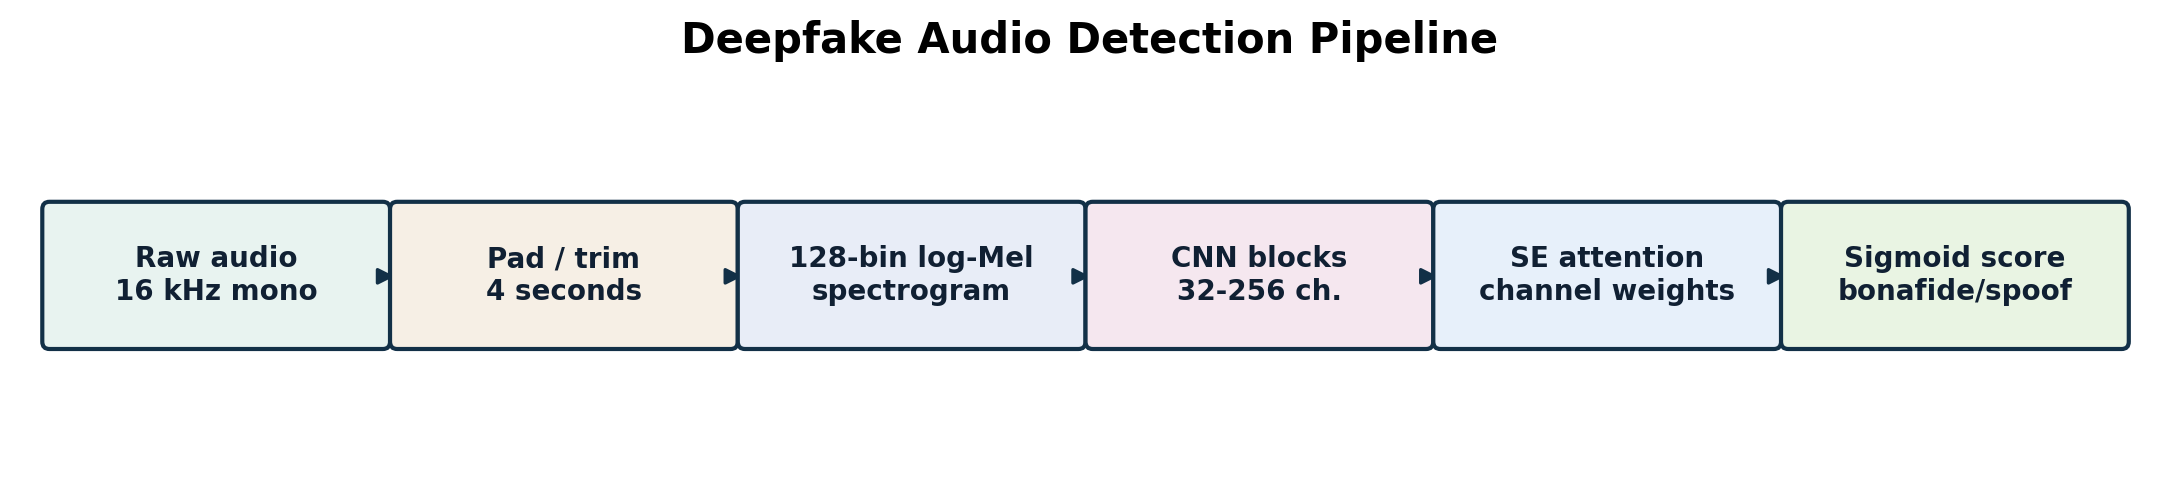
\includegraphics[width=0.95\linewidth]{system_pipeline.png}
    \caption{End-to-end deepfake audio detection pipeline. Raw audio is converted to a log-Mel spectrogram, fed through the convolutional stack and SE attention block, and reduced to a single sigmoid spoof score.}
    \label{fig:pipeline}
\end{figure}

\subsection{Model design}
My main model uses four convolutional blocks. Each block contains two $3\!\times\!3$ convolutions followed by batch normalization, ReLU activation, and $2\!\times\!2$ max-pooling. Channel depth grows from 32 to 64, 128, and 256. After the convolutional stack, a Squeeze-and-Excitation block with reduction ratio $r=16$ recalibrates the channels~\cite{hu2018senet}. The classifier head consists of global average pooling, a 512-unit fully connected layer with dropout, and a single logit unit. \Cref{fig:model} summarizes the architecture.

\begin{figure}[H]
    \centering
    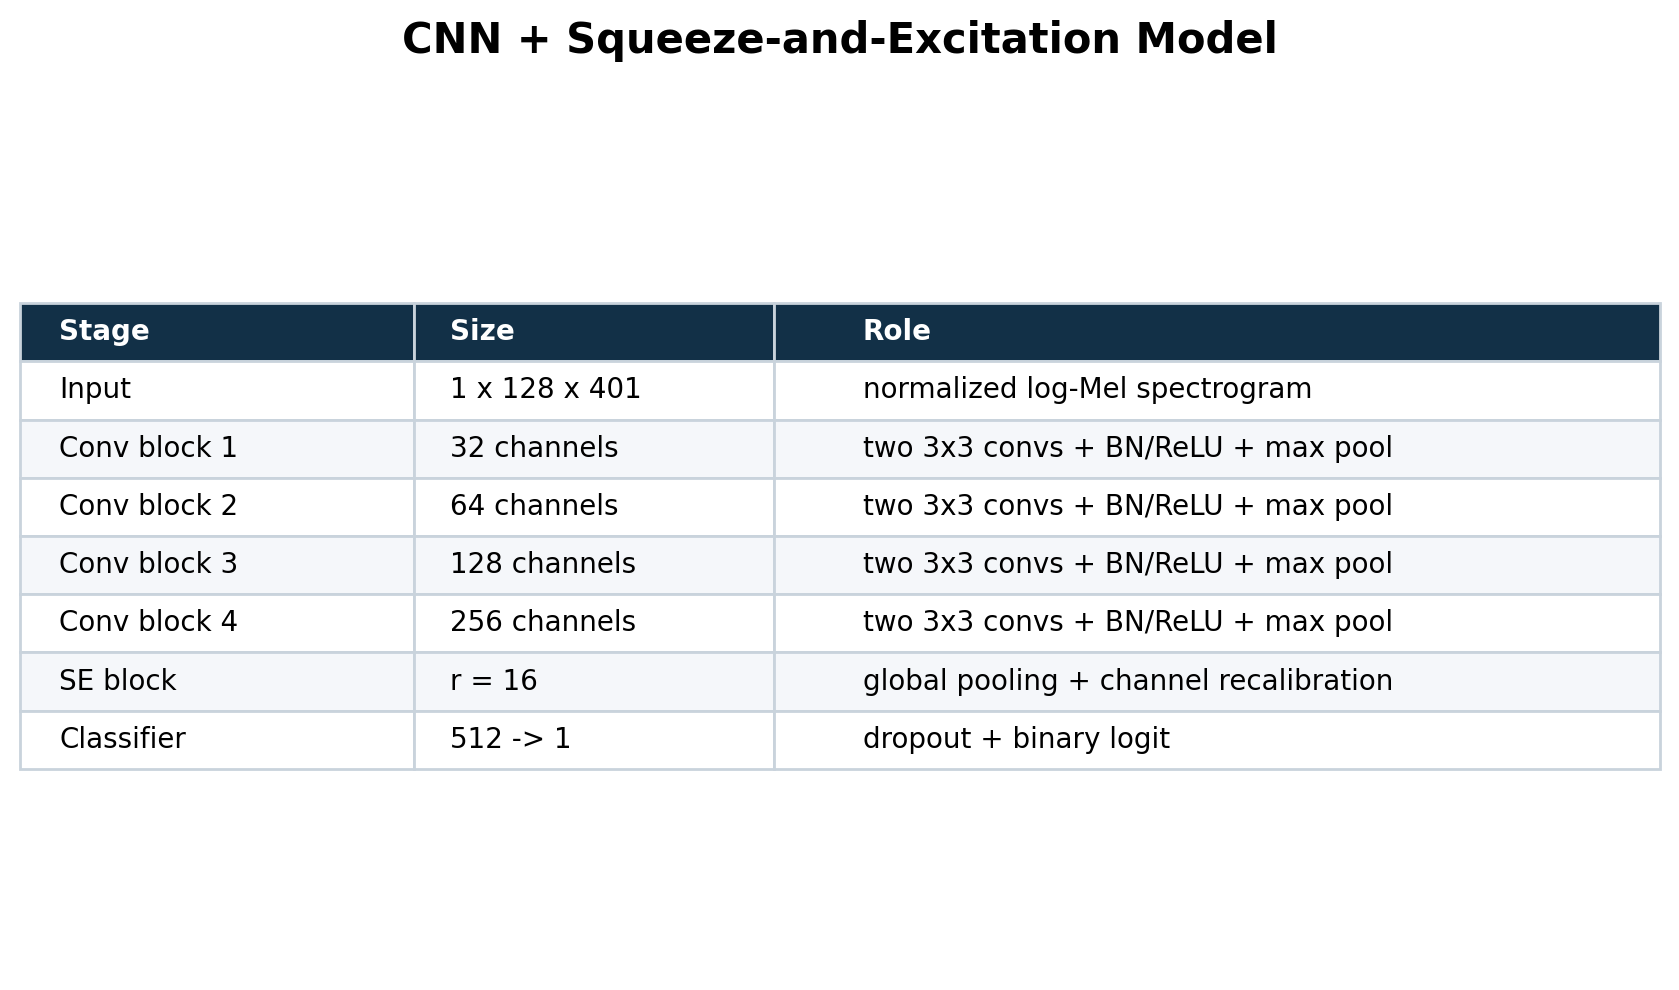
\includegraphics[width=0.86\linewidth]{model_architecture_table.png}
    \caption{CNN\,+\,SE architecture summary. Total parameter count: 1{,}312{,}929.}
    \label{fig:model}
\end{figure}

The CNN\,+\,SE model has $1.31\,\text{M}$ parameters; the ResNet-18 baseline has $11.17\,\text{M}$. That roughly $8\!\times$ size difference matters operationally, since a detector is more useful if it can run inside a podcast editing, review, or publishing workflow with negligible latency.

\subsection{Training details}
The neural detectors are trained with binary cross-entropy with logits, weighted by inverse class frequency. The eval set is heavily class-imbalanced (\(\approx 9{:}1\) spoof~:bonafide), and an unweighted loss can make the model lean too hard toward the majority class. I used Adam with initial learning rate $10^{-4}$ and cosine annealing across 30 epochs. Augmentation is applied to a random subset of the training batch and consists of additive background noise, synthetic room impulse responses, MP3 compression, and SpecAugment-style masking; pitch shifting is deliberately excluded so that channel and production effects, rather than artificial speaker-identity changes, drive the stress test. Best-checkpoint selection uses 2019 LA dev EER, not training loss, to avoid selecting an overfit checkpoint.

\paragraph{Hardware.}
All experiments were run locally on an Apple-Silicon MacBook through PyTorch's MPS backend. The reported per-clip latency is therefore a single-machine measurement and is not directly comparable to CUDA timings on dedicated server GPUs.

% =====================================================================
\section{Dataset and Preprocessing}\label{sec:data}

The experiment follows the standard ASVspoof Logical-Access protocol from the official challenge resources: train on ASVspoof 2019 LA train, tune on ASVspoof 2019 LA development, and evaluate on ASVspoof 2021 LA evaluation~\cite{asvspoof2019site,asvspoof2021site}. \Cref{tab:datasets} summarizes the splits used.

\begin{table}[H]
\centering
\caption{ASVspoof Logical-Access splits used in this study.}
\label{tab:datasets}
\small
\begin{tabular}{@{}lrrrl@{}}
\toprule
\thead{Split} & \thead{Bonafide} & \thead{Spoof} & \thead{Total} & \thead{Role} \\
\midrule
ASVspoof 2019 LA train & 2{,}580  & 22{,}800  & 25{,}380  & model fitting          \\
ASVspoof 2019 LA dev   & 2{,}548  & 22{,}296  & 24{,}844  & checkpoint selection   \\
ASVspoof 2021 LA eval  & 18{,}452 & 163{,}114 & 181{,}566 & final evaluation       \\
\bottomrule
\end{tabular}
\par\smallskip
{\footnotesize\itshape Note. The 2021 LA evaluation set contains spoofing systems A07--A19, none of which appear during training.}
\end{table}

\subsection{Preprocessing}
Every audio file passes through the same preprocessing path:
\begin{enumerate}
    \item load the waveform;
    \item convert to mono;
    \item resample to 16\,kHz;
    \item pad or trim to four seconds;
    \item compute a 128-bin log-Mel spectrogram (25\,ms Hann window, 10\,ms hop);
    \item normalize each spectrogram to zero mean and unit variance.
\end{enumerate}
The Mel-frequency warping reflects the perceptual scale of human hearing, and the log compresses the dynamic range that raw spectral magnitudes otherwise span.

\begin{figure}[H]
    \centering
    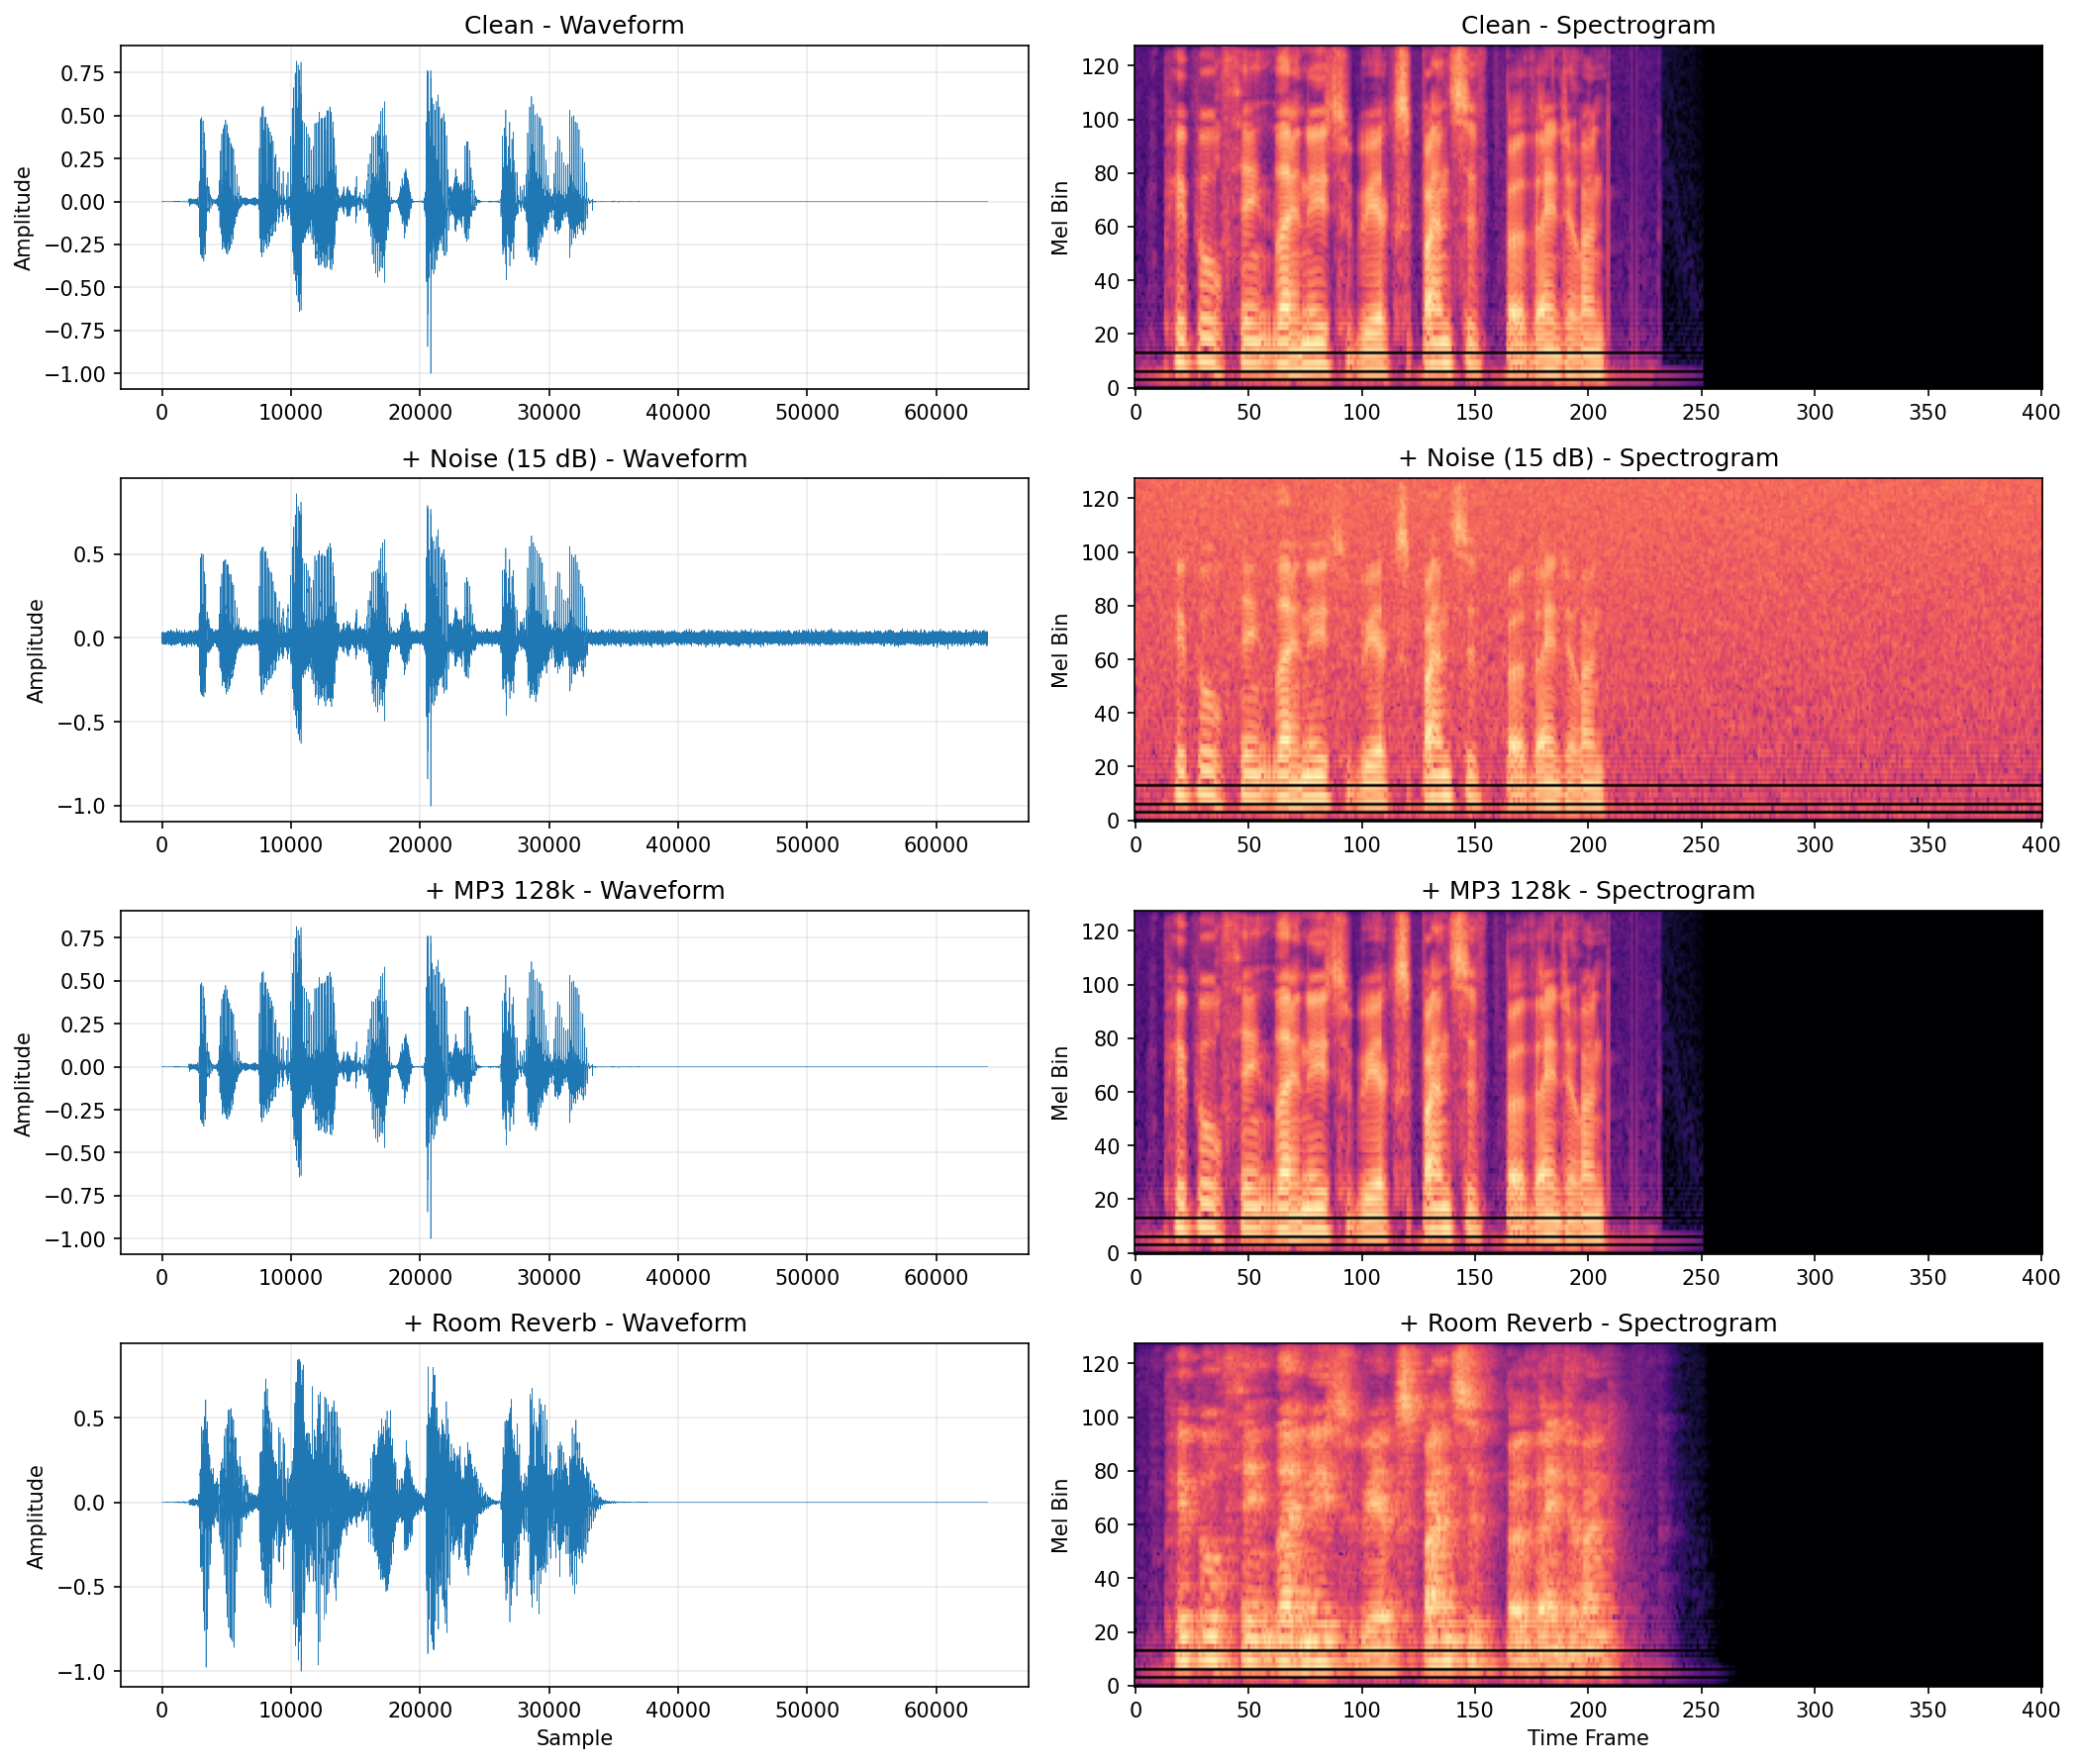
\includegraphics[width=0.95\linewidth]{augmentation_comparison_full.png}
    \caption{Example waveform and spectrogram views before and after podcast-style augmentation (room impulse response, additive background noise, and MP3 compression).}
    \label{fig:augmentation}
\end{figure}

\subsection{Cross-vocoder hold-out}
For the cross-vocoder diagnostic, a second CNN\,+\,SE model was trained with A05 and A06 spoofing samples removed from the 2019 training set; the held-out development check then evaluated on bonafide samples plus A05/A06 spoof samples. This isolates how well the detector ranks attacks it never saw during training.

% =====================================================================
\section{Experiments and Results}\label{sec:results}

\subsection{Evaluation metrics}
Equal Error Rate (EER) is the primary metric, because spoofing detection is fundamentally an operating-point problem. Accuracy is informative but can be misleading when the evaluation set is heavily imbalanced. AUC-ROC measures how well the continuous scores rank bonafide and spoofed examples regardless of threshold. Precision, recall, F1, and the confusion matrix all report the operating behavior at the fixed 0.5 threshold. Per-clip inference latency is also reported, since a usable podcast review tool cannot be slow.

\subsection{\texorpdfstring{Main CNN\,+\,SE result}{Main CNN+SE result}}
The CNN\,+\,SE model trained for 30 epochs on full 2019 LA train and selected its best checkpoint on full 2019 LA dev. The best development EER reached 0.0376\%. Although that is a useful sanity check, it should not be confused with final generalization: the meaningful test is the 2021 LA evaluation set, where the model must handle unseen attack systems and channel effects. \Cref{fig:training} shows the full training trajectory.

\begin{figure}[H]
    \centering
    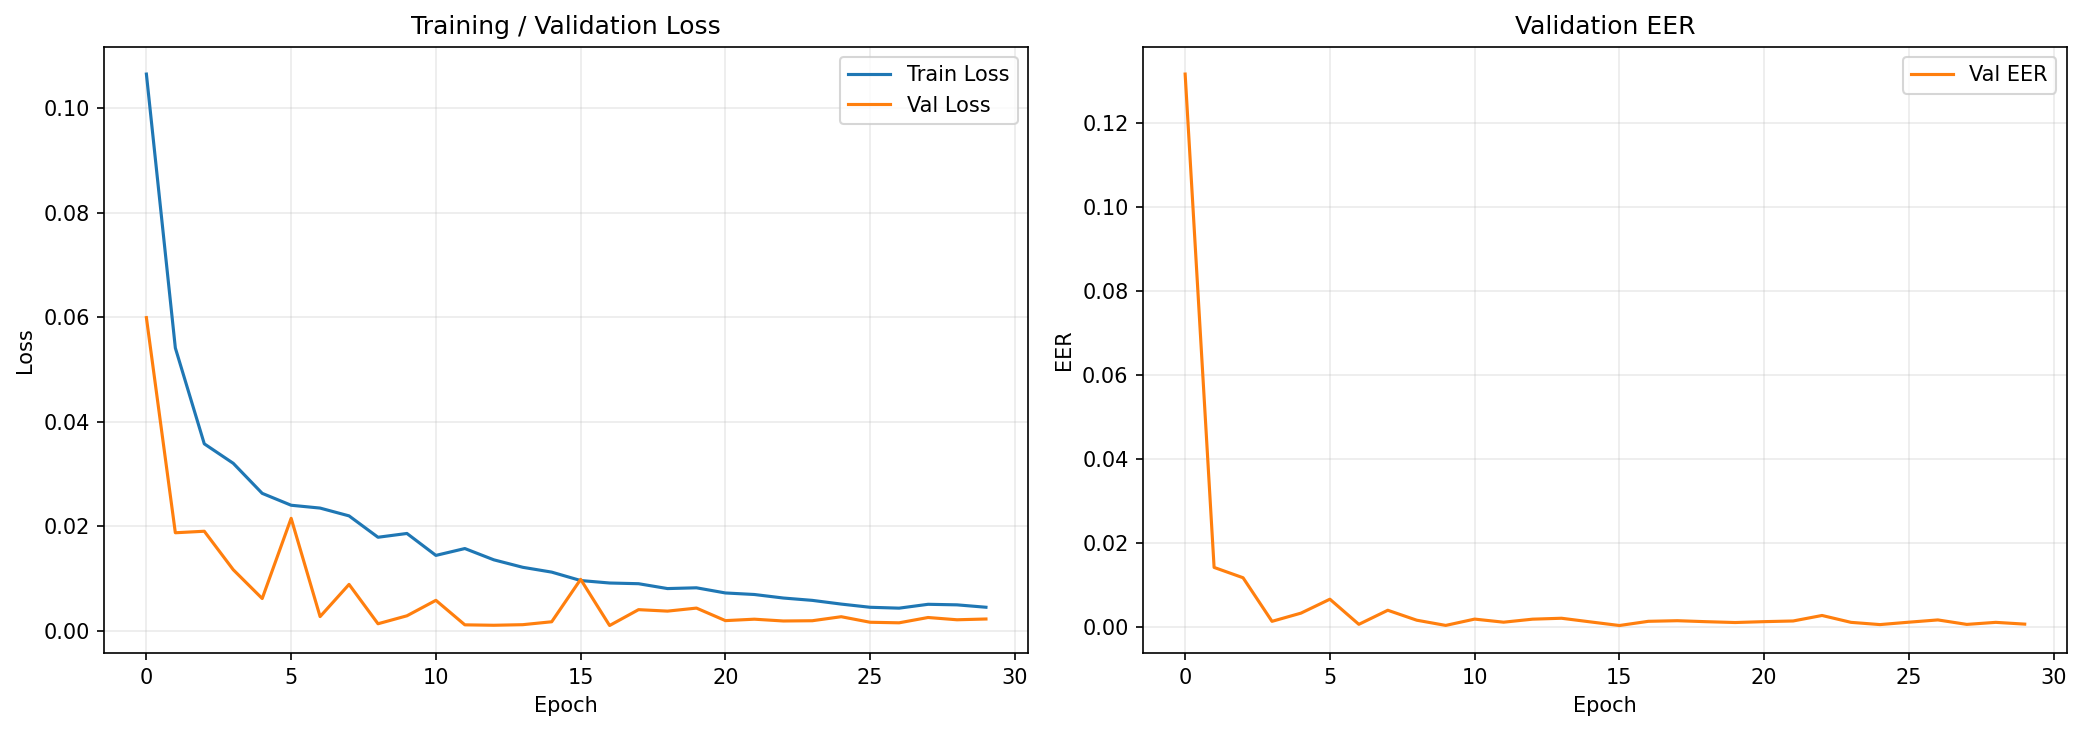
\includegraphics[width=0.86\linewidth]{training_history_full_cnn_se.png}
    \caption{Training history for the CNN\,+\,SE model. (a) train and validation loss; (b) validation EER on 2019 LA dev with the best checkpoint highlighted.}
    \label{fig:training}
\end{figure}

\Cref{tab:main} summarizes the headline results on full 2021 LA evaluation.

\begin{table}[H]
\centering
\caption{CNN\,+\,SE on full ASVspoof 2021 LA evaluation ($n=181{,}566$).}
\label{tab:main}
\small
\begin{tabular}{@{}lr@{}}
\toprule
\thead{Metric} & \thead{Value} \\
\midrule
Equal Error Rate (EER)        & 18.28\%  \\
AUC-ROC                       & 0.8979   \\
Accuracy at threshold 0.5     & 0.9072   \\
Precision at threshold 0.5    & 0.9567   \\
Recall at threshold 0.5       & 0.9392   \\
F1-score at threshold 0.5     & 0.9479   \\
Latency per 4\,s clip (MPS)   & 1.66\,ms \\
\bottomrule
\end{tabular}
\par\smallskip
{\footnotesize\itshape Note. EER and AUC use continuous scores; remaining metrics use threshold $=0.5$.}
\end{table}

The corresponding confusion matrix at threshold 0.5 is given in \cref{tab:cm}.

\begin{table}[H]
\centering
\caption{CNN\,+\,SE confusion matrix on clean 2021 LA at threshold 0.5.}
\label{tab:cm}
\small
\begin{tabular}{@{}l rr@{}}
\toprule
                & \thead{Predicted bonafide} & \thead{Predicted spoof} \\
\midrule
Actual bonafide & 11{,}517 & 6{,}935   \\
Actual spoof   &  9{,}922 & 153{,}192 \\
\bottomrule
\end{tabular}
\end{table}

The model performs well at the fixed 0.5 threshold (especially on recall and F1), but recall that the eval set is heavily spoof-skewed; the more security-relevant signal is the EER. At 18.28\% EER, the 2021 LA protocol is substantially harder than 2019 dev. \Cref{fig:roc} shows the ROC curve, which confirms that the model has learned a real ranking signal even when the chosen operating point is poor.

\begin{figure}[H]
    \centering
    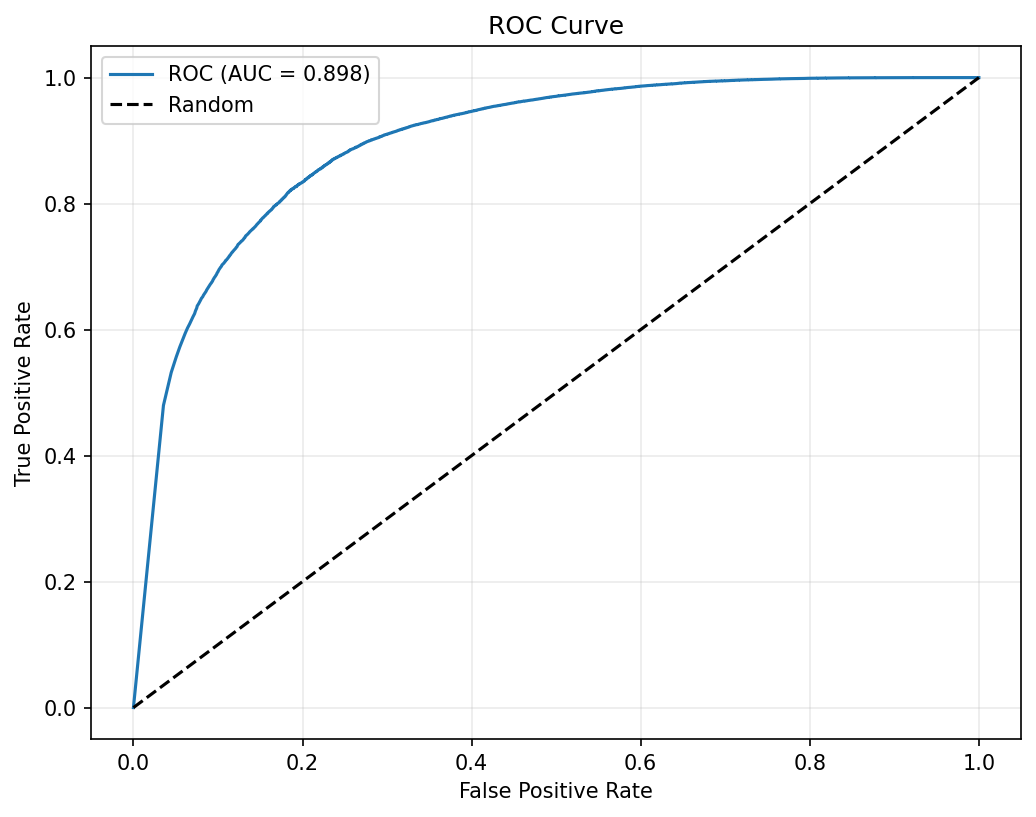
\includegraphics[width=0.65\linewidth]{roc_full_cnn_se_2021.png}
    \caption{ROC curve for CNN\,+\,SE on full ASVspoof 2021 LA. AUC-ROC $=0.8979$.}
    \label{fig:roc}
\end{figure}

\subsection{Podcast-style evaluation stress}
To stress-test the production side of the project, I re-evaluated the same checkpoint on the full 2021 LA eval set with podcast-style augmentation applied at evaluation time using a separate random seed. \Cref{tab:stress} compares the clean and stressed conditions.

\begin{table}[H]
\centering
\caption{Clean vs.\ podcast-style evaluation on ASVspoof 2021 LA.}
\label{tab:stress}
\small
\begin{tabular}{@{}lrrrrr@{}}
\toprule
\thead{Condition} & \thead{EER} & \thead{AUC-ROC} & \thead{Accuracy} & \thead{Recall} & \thead{F1} \\
\midrule
Clean 2021 LA              & 18.28\% & 0.8979 & 0.9072 & 0.9392 & 0.9479 \\
Podcast-augmented 2021 LA  & 18.48\% & 0.8852 & 0.8991 & 0.9301 & 0.9430 \\
\bottomrule
\end{tabular}
\end{table}

The augmented condition makes score separation slightly worse but does not collapse. EER moves from 18.28\% to 18.48\% (a $+0.2$\,pp shift) and AUC drops from 0.8979 to 0.8852. The model is robust enough to additive noise, room reverb, and MP3-style distortion to remain on-task, but the original below-10\% augmented-EER target is not met.

\subsection{Baseline comparison}
I compared the CNN\,+\,SE model against ResNet-18 trained on the same spectrogram pipeline and against a traditional LFCC-GMM baseline. \Cref{tab:baselines} summarizes the comparison on full 2021 LA evaluation.

\begin{table}[H]
\centering
\caption{Baseline comparison on ASVspoof 2021 LA evaluation.}
\label{tab:baselines}
\small
\begin{tabular}{@{}lrrrrrr@{}}
\toprule
\thead{Model} & \thead{EER} & \thead{AUC-ROC} & \thead{Accuracy} & \thead{F1} & \thead{Latency} & \thead{Params} \\
\midrule
\textbf{CNN\,+\,SE}            & 18.28\% & \textbf{0.8979} & \textbf{0.9072} & \textbf{0.9479} & \textbf{1.66\,ms} & \textbf{1.31\,M}  \\
ResNet-18                      & \textbf{17.21\%} & 0.8957 & 0.8549 & 0.9145 & 2.23\,ms & 11.17\,M \\
LFCC-GMM                       & 30.89\% & 0.7400 & 0.7063 & 0.8128 & n/a      & n/a      \\
\bottomrule
\end{tabular}
\par\smallskip
{\footnotesize\itshape Note. Latency measured on Apple Silicon MPS for a 4\,s clip. Bold marks the best result in each column.}
\end{table}

ResNet-18 attains the lowest EER at 17.21\%; my CNN\,+\,SE model does not win the headline metric outright. The honest interpretation is that ResNet-18 is the stronger detector on the security-relevant operating-point measure, while CNN\,+\,SE is competitive on AUC and stronger on threshold-dependent metrics at $0.5$, with roughly $8\!\times$ smaller capacity and lower per-clip latency. LFCC-GMM trails by approximately 13 EER points, providing the strongest evidence that learned spectrogram features capture spoofing cues that hand-crafted cepstra do not.

\subsection{Cross-vocoder hold-out}
The cross-vocoder experiment removed A05 and A06 spoofing systems from training and evaluated only on those held-out attacks during development. \Cref{tab:crossvoc} summarizes the result.

\begin{table}[H]
\centering
\caption{Cross-vocoder hold-out result on A05/A06 development split.}
\label{tab:crossvoc}
\small
\begin{tabular}{@{}lr@{}}
\toprule
\thead{Metric} & \thead{Hold-out A05/A06 dev} \\
\midrule
EER                          & 5.07\%  \\
AUC-ROC                      & 0.9881  \\
Accuracy at 0.5 threshold    & 0.4131  \\
Precision at 0.5 threshold   & 0.9962  \\
Recall at 0.5 threshold      & 0.2127  \\
F1 at 0.5 threshold          & 0.3506  \\
\bottomrule
\end{tabular}
\par\smallskip
{\footnotesize\itshape Note. Strong AUC and EER coexist with poor accuracy and F1 at threshold 0.5 because the score distribution shifts under attack-set hold-out. This is a calibration problem, not a ranking problem.}
\end{table}

This result requires careful interpretation. EER and AUC are both strong, indicating that the model separates the held-out systems well using the continuous score distribution. The fixed 0.5 threshold, however, is poorly calibrated for this split: the model becomes extremely conservative, almost never mislabels bonafide audio (precision 0.996), and consequently misses many spoof clips at the default decision boundary (recall 0.213). The practical lesson is that ranking quality and threshold quality are distinct properties and must be tuned independently.

% =====================================================================
\section{Discussion}\label{sec:discussion}

The project succeeds in the most important implementation sense: the full ASVspoof-style pipeline runs end-to-end. I trained on full 2019 LA train, tuned on full 2019 LA dev, evaluated on full 2021 LA, added a podcast-style stress evaluation, implemented two architecturally distinct baselines, and ran a cross-vocoder hold-out diagnostic. The downstream results, plots, checkpoints, and summary metrics are all reproducible from the released code.

The numerical results also illustrate why the problem is harder than the development split makes it look. The CNN\,+\,SE model reaches near-zero EER on 2019 dev, but that does not transfer directly to 2021 LA. The final 2021 EER of 18.28\% is well above the original below-5\% target and is not competitive with the top published ASVspoof 2021 systems. This is not a failure of the experimental procedure; it is an honest technical finding. A model can fit the 2019 development distribution very well and still struggle when codec conditions and unseen spoofing systems change.

Within the comparison to baselines, the picture is mixed. ResNet-18 obtains a lower EER (17.21\%) than CNN\,+\,SE and is therefore the stronger detector on the metric that matters most for security. CNN\,+\,SE is competitive on AUC (effectively tied at 0.898) and stronger on accuracy and F1 at threshold 0.5, but those threshold-dependent results should be treated cautiously because the cross-vocoder result demonstrates that 0.5 is the wrong operating point under distribution shift. The remaining argument for CNN\,+\,SE is operational: it runs at roughly $1/8$ the parameter count and lower per-clip latency, which matters in a near-real-time review setting.

The podcast-stress result is more positive than expected. EER moved only $+0.2$\,pp under additive noise, room impulse responses, and MP3 compression. That suggests the augmentation stack did not break the detector's basic decision surface, although it did slightly worsen ranking quality. The bigger weakness exposed by the experiment is generalization to the 2021 LA channel distribution, not augmentation robustness per se.

\paragraph{Limitations.}
The main limitations are: (i)~the podcast-style augmentation is synthetic and does not model the full digital-audio-workstation export chain (EQ, dynamic-range compression, broadcast loudness normalization, platform re-encoding); (ii)~the fixed 0.5 threshold is empirically poorly calibrated under distribution shift, so threshold-dependent metrics should be interpreted with care; (iii)~the latency number is a single-machine measurement on Apple-Silicon MPS and does not constitute a hardware-versus-hardware claim; (iv)~the original below-5\% clean-EER target is not met, so the detector is not appropriate for unsupervised production deployment without further work.

% =====================================================================
\section{Conclusion and Future Work}\label{sec:conclusion}

This project implements a spectrogram-based CNN with Squeeze-and-Excitation attention for deepfake-audio detection in podcast production, runs the full ASVspoof-style protocol from training through evaluation, and reports honest results, plots, and metrics. The main takeaways are:
\begin{itemize}
    \item CNN\,+\,SE learns useful spoofing signals from log-Mel spectrograms but does not yet generalize strongly to the full 2021 LA protocol.
    \item Podcast-style stress did not break the detector, but it did slightly lower its score-ranking quality.
    \item ResNet-18 attained the lowest EER, while CNN\,+\,SE offered a more favorable size, latency, and threshold-dependent-metric trade-off.
    \item Threshold calibration matters substantially under cross-vocoder hold-out and other distribution-shift conditions.
\end{itemize}

The natural continuations of this work are:
\begin{enumerate}
    \item calibrate decision thresholds on production-style validation data rather than relying on the default 0.5;
    \item evaluate against real podcast export chains taken directly from a digital audio workstation, to replace the synthetic augmentation surrogate;
    \item benchmark on additional hardware where runtime claims are operationally relevant;
    \item try stronger anti-spoofing models, including RawNet-style and transformer-based detectors;
    \item add explainability views (e.g.\ Grad-CAM on log-Mel spectrograms) so that human reviewers can understand which time-frequency regions drove a given spoof decision.
\end{enumerate}

\paragraph{Reproducibility.}
All code, checkpoints, metrics, and figure-rendering scripts referenced in this report are in the public \href{https://github.com/brianstever/APCV485_Final_Project_Stever}{GitHub repository}. The presentation PDF and notebook walkthrough are included in the submitted repository folder.

% =====================================================================
\bibliographystyle{ieeetr}
\begin{thebibliography}{13}

\bibitem{wang2020asvspoof2019}
X.~Wang \emph{et al.}, ``ASVspoof 2019: A large-scale public database of synthesized, converted and replayed speech,'' \emph{Computer Speech \& Language}, vol.~64, article 101114, 2020, doi: 10.1016/j.csl.2020.101114.

\bibitem{liu2023asvspoof2021}
X.~Liu \emph{et al.}, ``ASVspoof 2021: Towards spoofed and deepfake speech detection in the wild,'' \emph{IEEE/ACM Trans.\ Audio, Speech, Lang.\ Process.}, vol.~31, pp.~2507--2522, 2023, doi: 10.1109/TASLP.2023.3285283.

\bibitem{todisco2017cqcc}
M.~Todisco, H.~Delgado, and N.~Evans, ``Constant Q cepstral coefficients: A spoofing countermeasure for automatic speaker verification,'' \emph{Computer Speech \& Language}, vol.~45, pp.~516--535, 2017, doi: 10.1016/j.csl.2017.01.001.

\bibitem{sahidullah2015features}
M.~Sahidullah, T.~Kinnunen, and C.~Hanil\c{c}i, ``A comparison of features for synthetic speech detection,'' in \emph{Proc.\ Interspeech 2015}, pp.~2087--2091, 2015, doi: 10.21437/Interspeech.2015-472.

\bibitem{tak2021rawnet2}
H.~Tak, J.~Patino, M.~Todisco, A.~Nautsch, N.~Evans, and A.~Larcher, ``End-to-end anti-spoofing with RawNet2,'' in \emph{Proc.\ IEEE International Conference on Acoustics, Speech and Signal Processing (ICASSP)}, pp.~6369--6373, 2021, doi: 10.1109/ICASSP39728.2021.9414234.

\bibitem{lai2019assert}
C.-I.~Lai, N.~Chen, J.~Villalba, and N.~Dehak, ``ASSERT: Anti-Spoofing with Squeeze-Excitation and Residual neTworks,'' arXiv:1904.01120, 2019, doi: 10.48550/arXiv.1904.01120.

\bibitem{hu2018senet}
J.~Hu, L.~Shen, and G.~Sun, ``Squeeze-and-Excitation Networks,'' in \emph{Proc.\ IEEE Conference on Computer Vision and Pattern Recognition (CVPR)}, pp.~7132--7141, 2018, doi: 10.1109/CVPR.2018.00745.

\bibitem{park2019specaugment}
D.~S. Park, W.~Chan, Y.~Zhang, C.-C.~Chiu, B.~Zoph, E.~D.~Cubuk, and Q.~V.~Le, ``SpecAugment: A simple data augmentation method for automatic speech recognition,'' in \emph{Proc.\ Interspeech 2019}, pp.~2613--2617, 2019, doi: 10.21437/Interspeech.2019-2680.

\bibitem{he2016resnet}
K.~He, X.~Zhang, S.~Ren, and J.~Sun, ``Deep residual learning for image recognition,'' in \emph{Proc.\ IEEE Conference on Computer Vision and Pattern Recognition (CVPR)}, pp.~770--778, 2016, doi: 10.1109/CVPR.2016.90.

\bibitem{yi2023survey}
J.~Yi, C.~Wang, J.~Tao, X.~Zhang, C.~Y.~Zhang, and Y.~Zhao, ``Audio deepfake detection: A survey,'' arXiv:2308.14970, 2023, doi: 10.48550/arXiv.2308.14970.

\bibitem{nautsch2021asvspoof}
A.~Nautsch \emph{et al.}, ``ASVspoof 2019: Spoofing countermeasures for the detection of synthesized, converted and replayed speech,'' \emph{IEEE Transactions on Biometrics, Behavior, and Identity Science}, vol.~3, no.~2, pp.~252--265, 2021, doi: 10.1109/TBIOM.2021.3059479.

\bibitem{asvspoof2021site}
ASVspoof Consortium, ``ASVspoof 2021 challenge website and database resources,'' accessed May~3, 2026. [Online]. Available: \url{https://www.asvspoof.org/index2021.html}

\bibitem{asvspoof2019site}
ASVspoof Consortium, ``ASVspoof 2019 challenge website and database resources,'' accessed May~3, 2026. [Online]. Available: \url{https://www.asvspoof.org/index2019.html}

\end{thebibliography}

\end{document}
